\documentclass[a4paper,%
	12pt,%
	DIV14,
	headsepline,%
	headings=normal,
]{scrartcl}
\usepackage[utf8]{inputenc}
\usepackage[T1]{fontenc}
\usepackage{textcomp}

\usepackage{color}
\usepackage{hyperref}
\usepackage{graphicx}
\usepackage{listings}
\usepackage[hang, font = footnotesize]{caption}
\usepackage{algorithm}
\usepackage{enumitem}
\usepackage{amssymb}
\usepackage{amsmath}
\usepackage{mathtools}
\usepackage{amsthm}
\usepackage{mathrsfs}
\usepackage{mathalpha}
\usepackage{wrapfig}
\usepackage{subcaption}



\newtheorem{theorem}{Theorem}
\newtheorem{lemma}[theorem]{Lemma}
\newtheorem{corollary}[theorem]{Corollary}
\theoremstyle{definition} 
\newtheorem{definition}[theorem]{Definition}
\theoremstyle{remark}
\newtheorem{remark}[theorem]{Remark}
\newtheorem{comment}[theorem]{Comment}
\newtheorem{solution}{Solution}


\lstset{language=C++,
basicstyle=\small\ttfamily,
keywordstyle=\color{blue}\ttfamily,
stringstyle=\color{red}\ttfamily,
commentstyle=\color{green}\ttfamily,
morecomment=[l][\color{magenta}]{\#},
numbers=left, numbersep=5pt, tabsize=4,
}

\begin{document}
\hrule height 1px
\vspace*{2ex}

\begin{center}
	{\Huge Research Proposal for Master's Thesis}\\
	\vspace{2mm}
	
	{\large An efficient set union operation on distributed memory machines} \\
	\vspace{10mm}
		
	{\Large Frieder Wolpert-Veit} \\
	{12135828}\\
	\vspace{6mm}
	
	{\Large 2026} \\
	\hspace{3mm}
\end{center}
\hfill

\hrule 
\vspace{4mm}

This research proposal introduces a topic for the Master's thesis titled '\emph{An efficient set union operation on distributed memory machines}'. For this firstly the research field is explained to get some context in which kind of field this thesis aims at. Next a motivation is given which leads to an explicit problem statement. Then an overview is given that covers related work relevant for the problem statement. After this a research gap is identified and it is stated how the proposed thesis contributes to expand the research field. With this there are also explicit research questions articulated. The later sections cover the intended methodology to and which results/limitations can be expected.

\section{Research field}
The topic of the proposed thesis is part of the research field \emph{Parallel Computing}/\emph{High Performance Computing}. Explicitly it is part of \emph{Distributed Memory Computing}. In distributed memory computing machines are used that are built out of multiple processors which generally do not have access to a shared memory space. Typically, these machines are clusters of compute nodes with each node  holding multiple processors. The compute nodes are connected with each other with some kind of interconnect. To perform parallel computing on such clusters multiple processes are executed (typically one per processor) and communication is only possible by sending messages between processes. As framework for handling this communication the Message Passing Interface (MPI) \cite{mpi} is the de-facto standard. This interface allows sending messages between two processes (point-to-point communication) and also provides useful procedures where multiple processes participate (collective communication). \cite{lecturesTräff, modelDistributedMemory}\\
MPI is only a standard which is implemented by different libraries like OpenMPI, MPICH or IntelMPI. How different (especially collective) procedures are implemented is an active research field \cite{traeff2025}.

\section{Motivation}
The problem which will be stated in the next section is motivated by the aim of finding an efficient building block to perform a Breath-First-Search (BFS) on distributed memory machines. A BFS is an algorithm where a graph is iteratively explored. For this a node of the graph is selected as starting  point (called root). In the first iteration of the BFS is the neighborhood of root node explored. In the next iteration the neighborhood of this neighborhood and so on. \cite{standardBFS, introToAlgos}\\
There are different approaches how such a BFS can be executed efficiently on a distributed memory machine. All the approaches have in common that the considered graph is distributed to the different processes. There are approaches that distribute the nodes of the graph to the processes \cite{graphPartitioning, hybridBFS}. We consider here a variant where the set of edges is portioned and each process takes care of an approximately equal amount of edges. The strategy is to spread the workload in each iteration of the BFS equally over all process to find the next neighborhood. Calling the current explored neighborhood 'frontier', each process finds in this approach in each iteration vertices of the new frontier that can be found by its available edges. After that each process holds a subset of the new frontier. For the next iteration the frontier must be available for all processes and therefore a union of all the subsets needs to be calculated. The development of an efficient algorithm to calculate such a union operation is the aim of the proposed thesis.

\section{Problem statement}
The aim of the thesis is to efficiently calculate a union of sets that are distributed over different processes. The subsets are here subsets of a given universe set. Also, there is the condition that the calculated union must be available to all processes and not just to one.\\
Formally, we look for an efficient way such that each process calculates 
\begin{align*}
	U = \bigcup_r S_r
\end{align*}
where $S_r$ is the proposed set by process $r$. For all these sets holds $S_r\subseteq \Tilde{S}$ with $|\Tilde{S}|$ being finite.

\section{Related work}
One important part is how the sets $S_r$ are represented at the processors. For this it is useful to label all elements of $\Tilde{S}$ from $0$ up to $|\Tilde{S}|-1$. One representation for a set is to create a list of integers that holds all elements that are in the set. To get the union $U$ of all sets $S_r$ all lists representing $S_r$ need to be concatenated. This can lead to element duplicates which can be removed later or left in place redundantly. This representation will be called here \emph{sparse} representation. \\
Another way of representing sets is using a bitmap. As the universe set $\Tilde{S}$ is of finite size an array consisting out of $|\Tilde{S}|$ can be created where bits are set to 1 where corresponding elements are in the set $S_r$. Bits that correspond to elements that are not in $S_r$ are set to $0$. This representation  will be called here \emph{dense} representation. To calculate a union two such bitmaps need to be combined using a bitwise OR. \cite{graphPartitioning}\\
The sparse representation is beneficial if there are only a few elements in each $S_r$ as only a few integers are needed to save a whole set $S_r$. A reasonable integer type takes 32 bits of memory. The memory footprint grows therefore linearly with the filling of the sparse representations. The dense representation on the other hand is only dependent on the size of the universe set $|\Tilde{S}|$. It takes only one bit per element of $|\Tilde{S}|$. One can see that there is a point for largely filled sets $S_r$ where the dense representation is more efficient on the memory than the sparse one.
\subsection{Procedures that perform a union}
There are already procedures that can be used to perform a union on the sets for either of the representations. The sparse representation needs a procedure that concatenates all sparse lists and makes this list available to all processors. This procedure is provided by MPI by the collective communication procedure \emph{Allgather} \cite{mpi}. There are many algorithms available that explicitly implement an Allgather \cite{allgather}. \\
To calculate a union of densely represented sets an \emph{Allreduce} is needed \cite{graphPartitioning}. For an Allreduce each process proposes a value and as a result the sum over all these inputs is returned. The term 'sum' is here used quite loosely and refers to the combination of all inputs with respect to an associative operator \cite{mpi}. When performing an Allreduce using a bitwise OR as operator a union can be logically achieved. There also many algorithms available that implement an Allreduce \cite{AllreduceSummaryAll}. \\
There are also theoretical frameworks available that can be used to estimate execution times of point-to-point and collective communication algorithms. One of the simplest but still relevant frameworks is the \emph{linear cost model} \cite{costModels, hockneyLinearCostModel}. Here it is assumed that the time to send a message of size $m$ (in bits) from one process to another can be calculated by $T=\alpha + \beta m$. The parameter $\alpha$ and $\beta$ are dependent on the system the send is executed on. This model will be used in the proposed thesis to estimate execution times of the discussed Algorithms.
\subsection{Data compression for MPI}.
In the next section it is proposed that algorithms will be developed for this thesis that uses both (sparse as well dense) representations. This can be interpreted as a kind of data compression to minimize communication costs on the distributed memory machine. It is important to mention that a similar approach of sparsely and densely represented sets is already used in the context of shared memory computing. The LIGRA framework proposed by Shun et al. provides an interface to build graph traversal  algorithms (like BFS) where sets are represented densely as well as sparsely to improve performance \cite{Ligra}.\\
There are different ideas how to use some kind of data compression to accelerate collective communication on distributed memory machines \cite{compOnlinePipelining, compCountSketchAllreduce, compQuantizationAndSparseAllred}. These research is here mainly focused on a global summation (An Allreduce using $+$ as binary operator) of floating point arrays as this is a relevant set in the training process of statistical models like artificial neural networks. The approach that is most similar to the ideas proposed in this article is done by Rengli et al. \cite{compSparseDense}. They use sparsely represented arrays to perform an efficient summation of floating point arrays.

\section{Research gap and aim of the thesis}
The main aim of the proposed thesis is the development of algorithms that perform a union operation. These algorithms are built in a way that they dynamically switch between a dense and sparse representation such that the more efficient format is chosen. To realize such algorithms two properties are identified. Firstly it is known that some quite well performing Allreduce implementations are built out of a Reducescatter followed by an Allgather \cite{AllreduceSummaryAll}. The second important property is that the communication pattern of the Reducescatter is quite similar and sometimes even identical to that of an Allgather. The idea is therefore to overlay a dense Reducescatter phase of an Allreduce over an Allgather on sparse representations. Depending on the filling of the proposed sets the algorithm behaves more like an Allreduce (if sets are heavily filled) or more like an Allgather (if sets are sparsely filled).\\
The aim is to build two different algorithms that capitalize on this idea. The first one only is required to work for a number of processes that is a power of two and the second one does not have this constraint. There is a reason to include an extra version where the number of processors is constrained to be a power of two. We expect a performance gain as this algorithm will exploit architectural properties for systems that are built out of compute nodes that each hold a number of processors that is a power of 2. For these systems there are communication patterns where for a part of the execution communication only happens between processors that sit physically on the same compute node.\\
With this overall aim we formulate specific research questions for the thesis:
\begin{itemize}
	\item Are there indeed regimes where the newly proposed algorithms outperform a setup where only a sparse Allgather/ only a dense Allreduce is used?
	\item How close is the performance of the newly proposed algorithms compared native MPI variants
	\item How do different system setups influence the execution time? 
	\item Are the new union operations useful in the context of building a BFS? 
\end{itemize}

\section{Methodology}
The new union algorithm are analyzed theoretically and experimentally. Both these requirements hold validating correctness and the estimating/measuring the performance of the algorithms. \\
To show theoretical correctness there are proofs validating that the new union algorithms perform indeed a union operation. There are also proofs provided for algorithms the newly proposed procedures are built upon. To estimate the performance of the new implementations the linear cost model is used. With this a comparison against naive variants (meaning implementations that only use a dense/sparse representation) will be done.\\
\subsection{Experimental testing}
To validate and benchmark implementations a small cluster at TU Wien is available. It consists out of 36 compute nodes which are connected via dual Intel\textsuperscript{\textregistered} Omni-Path interconnect. Each node is equipped with two Intel\textsuperscript{\textregistered} Xeon\textsuperscript{\textregistered} Gold 6130F 16-Core CPUs. All testing is performed on this machine.\\
The correctness of the implementations will also be tested experimentally. For this are unit tests executed. Moreover, the union algorithm will be used as a building block of an BFS implementation to test for a correct behavior.\\
On the other hand there is a main focus on the evaluation of the performance of the new Algorithms.
Firstly the algorithms that build the foundation of the newly proposed algorithms are tested and a setup is found where these algorithms are the fastest. For this, different MPI libraries (OpenMPI, IntelMPI and MPICH) are used. Also, the number of processors and their layout on the nodes is varied. Secondly the new algorithms are compared against their foundation algorithms. This is done for different processor layouts and with varying setup parameter (like the size of the universe set $|\tilde{S}|$ and how much the sets are filled). Thirdly the performance of the newly proposed algorithms are tested in the application of a BFS. As reference serves an implementation that relies only on densely represented sets and uses an Allreduce to perform a union operation.\\
The measuring methodology is closely oriented at the work of Hunold and Carpen-Amarie \cite{HunoldBench}. The benchmark setup is using a \textbf{for}-loop with one execution of the parallel program to test different parameter settings multiple times. This allows to preprocess
the data and omit statistical outliers. The important part is to execute these hole procedure multiple times to obtain statistically sound results.

\section{Expectations and limitations}
We expect that is possible that it is possible to build two algorithms which are up to a linear constant as fast as the better version between an implementation that solely relies on either a sparse Allgather or a dense Allreduce. Formally, the execution time of the new union algorithms $T$ is expected to be bound by
\begin{align*}
	T \leq \kappa \min(T_\mathrm{Allgather}, T_\mathrm{Allreduce})
\end{align*}
with $\kappa$ being some constant, $T_\mathrm{Allgather}$ the execution time of an implementation using only an Allgather and $T_\mathrm{Allreduce}$ the execution time of an implementation using only an Allreduce. So for low set fillings the newly proposed algorithms are expected to behave more like an Allgather and for high set fillings more like an Allreduce. 
\begin{figure}
	\centering
	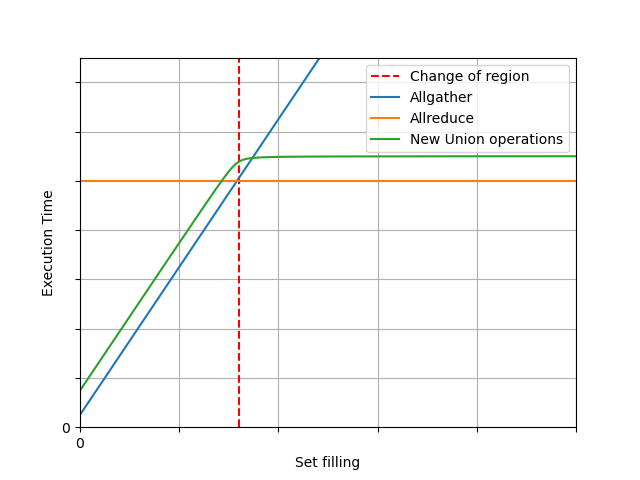
\includegraphics[width=0.7\textwidth]{../plots/Expose/runtimeSchematic.png}
	\caption{Expected run times of an Allgather and Allreduce implementation compared to the newly proposed algorithms.}
	\label{fig:runtimeSchematic}
\end{figure} 
Figure \ref{fig:runtimeSchematic} shows schematically how we expect the execution times of the different implementations relate to each other. Here the dashed red line marks separates the regions where an Allgather is more efficient or an Allreduce is preferred. Just by comparing the memory footprint of the sparse representation with the dense one we expect this separation to be when the resulting union represents a set that is filled with $\frac{|\tilde{S}|}{I}$ elements. Variable $I$ marks here the memory footprint of the integer that are used for the sparse representation. With an integer size of 32 bits the expected region where an Allgather is more efficient is when the resulting set is filled with around $3\%$ of the universe set $\Tilde{S}$.\\
With this in mind, we expect that there are setups where the new union algorithms improve the performance of a BFS. During a BFS are the frontier sizes of the first and the last iterations quite small. For the other iterations the frontier can be quite large. Therefore, we expect a system that dynamically switches representations to perform better than one that relies only on either the sparse representation or the dense one. The limitation is here that the actual size of the frontiers depend on the graphs the BFS is executed on. So the expected amount of gain depends on it. There could also be graphs for which the newly proposed algorithms build an BFS implementation that is slower than one of the references.\\
The thesis will mainly compare the newly proposed algorithms against foundation (Allgather/Allreduce) algorithms that are implemented by the researcher. This is done to identify which beneficial or detrimental effects stem from the algorithmic behavior and to exclude effects that stem from the actual implementation. It could be that native functions provided by well-developed MPI libraries still perform better.\\
Another aspect is that we develop these algorithms to provide the best performance on the given physical setup. Even with changing and analyzing different processor layouts it could be that we optimize only for systems that are build similarly. 


\newpage
\bibliographystyle{alpha}
\bibliography{references}
\end{document}




















